\graphicspath{{chapters/_resources/}}

\chapter{Telomeres and telomere transcription in cancer}

\hypertarget{what-are-telomeres}{%
\subsection{What are telomeres?}\label{what-are-telomeres}}

A DNA double strand break (DSB) generates new chromosome ends, which are
structurally similar to a telomere. But what is so special about the
extremities of our chromosomes?

Telomeric DNA is made of \emph{telomeric repeats}, 2-20kb in length and
forming GC rich sequences (seen when talking about R-loops). They depend
on the current cell cycle phase. A few nucleotides before telomeres we
find \emph{subtelomeric repeats} (''patchwork'' sequences duplicated
during evolution, devoid of genes and less conserved).

\textbf{Study from Barbara McClintock}: she treated chromosomes with
X-Rays and she observed large chromosomal aberrations, since breaks can
be repaired by the fusion among different chromosomes. However, she
noticed that such fusions never occurred between extremities. Somehow
the physiologic ends of chromosomes were protected from these fusions.
Even if chromosomes end with the exact same sequence, there are no
identical extremities, as the t-loop can invade in different positions.

\hypertarget{telomeres-mask-chromosome-ends-from-being-recognized-as-double-strand-breaks}{%
\subsubsection{Telomeres mask chromosome ends from being recognized as
double-strand
breaks}\label{telomeres-mask-chromosome-ends-from-being-recognized-as-double-strand-breaks}}

Telomeres form t-loops: mammalian telomeres end in a large loop. A
T-loop does not form by itself, but some proteins are involved. In
particular, TRF2 dimer facilitates the strand invasion - in fact
telomeres t-loops are TRF2 dependent.

Telomeric DNA is coated with telomere binding proteins → \emph{shelterin
complex}: It contains: TRF1 and TRF2 (dsBP), POT1 (ssBP), RAP1, TIN2 and
TPP1 (bridging). The complex allows dsbp and ssbp to interact. We know
that there are also subcomplexes on telomeres.

\begin{figure}
\centering
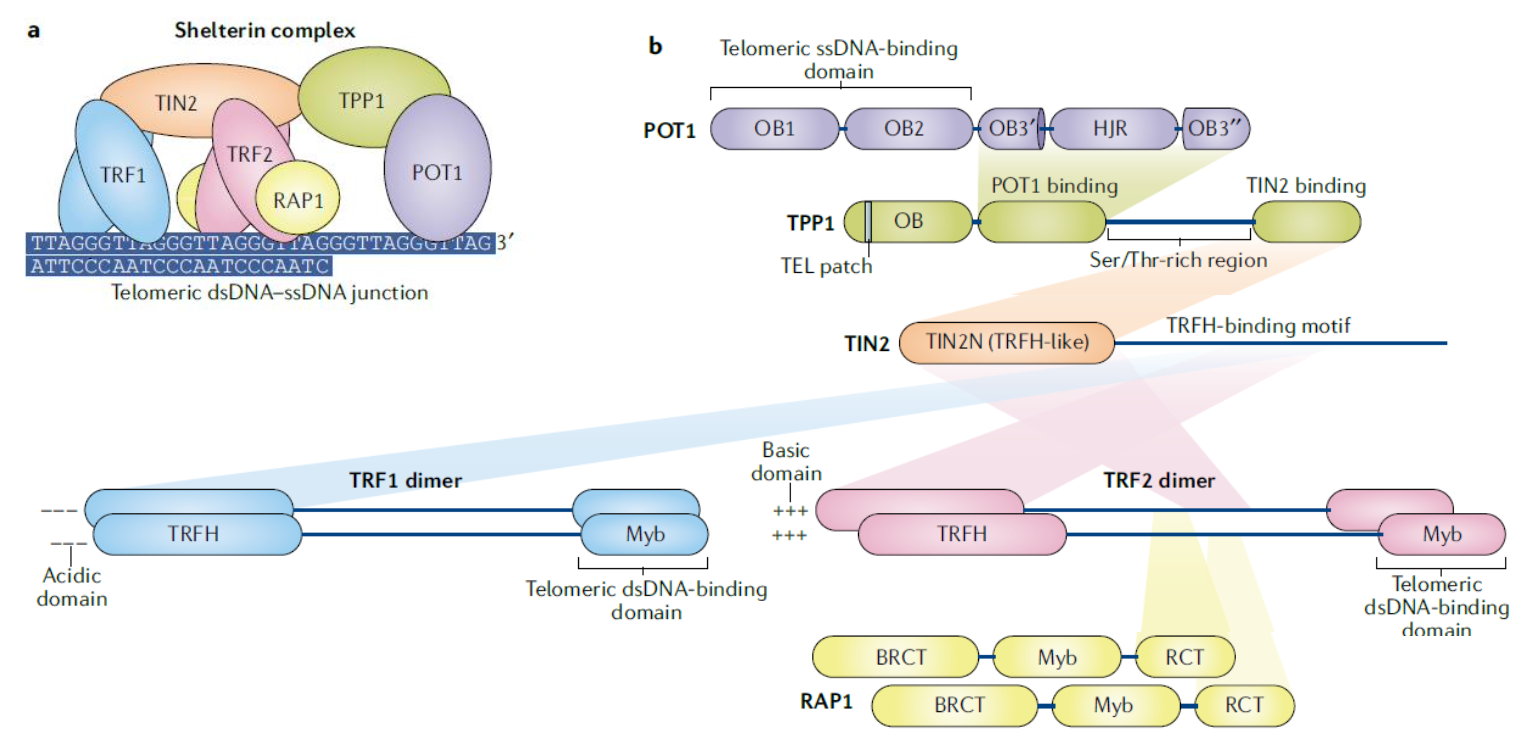
\includegraphics[width=0.5\textwidth]{../_resources/Screen_Shot_2022-12-15_at_17-43-24.png}
\caption{Lim and Cech, Nature Reviews Mol Cell Biol, 2021}
\end{figure}

Lim and Cech, Nature Reviews Mol Cell Biol, 2021

What is the function of this complex? Expression of a dominant negative
form of TRF2 (TRF2 B M), which is unable to bind telomeres, destabilizes
the shelterin complex. By removing the basic and main domain of the
stabilizing complex, the complex is disassembled. Telomere dysfunction
results in activation of DNA damage response at telomeres. Cells stop
dividing with this treatment, if the DDR pathway works correctly. The
impaired telomere structure induces DDR at chromosome ends leading to
dysfunctional telomeres.

TRF2 inhibits the recruitment of ATM through the formation of the t-loop
and then there's POT1, which represses the ATR pathway. POT1 can
displace RPA, which is not recruited and cannot interact with ssDNA.

\hypertarget{telomere-dysfunction-in-a-p53-and-rb-mutant-setting-does-not-induce-cell-cycle-block}{%
\subsection{Telomere dysfunction in a p53 and Rb mutant setting does not
induce cell cycle
block}\label{telomere-dysfunction-in-a-p53-and-rb-mutant-setting-does-not-induce-cell-cycle-block}}

Dysfunction of telomeres induces cell apoptosis through the usual P53-
and ATM Dependent pathways. Problem: in cancer the apoptosis pathways
are often impaired.

IMR90 (Human Lung fibroblast), cell line HT1080 (sarcoma cell line) →
repress Cdk6, activate Cdk1. P53/Rb mutant cells continue dividing
despite the presence of dysfunctional telomeres! (gammaH2X)

Telomeres detected by DNA FISH on chromosome spread nicely co-localize
at chromosome ends in untreated IMR90 E6E7 cells. If we apply TRF2
depletion, we observe something different.

\begin{figure}
\centering
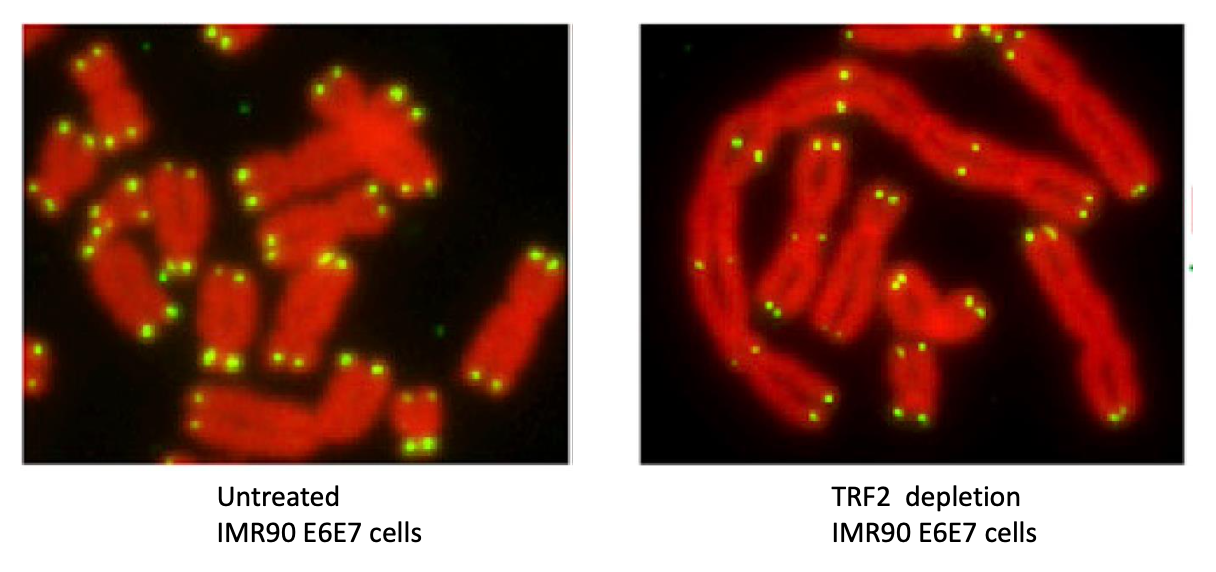
\includegraphics[width=0.5\textwidth]{../_resources/Screen_Shot_2022-12-15_at_17-54-31.png}
\caption{Cesare \emph{et al., Mol Cell} 2013}
\end{figure}

Cesare \emph{et al., Mol Cell} 2013

While the DNA damage response is not active, DNA repair pathways are
still active: cells continue proliferating and activating repair
mechanisms (in particular NHEJ) for what is perceived as a DSB. This
results in the fusion of chromosome ends → source of massive
\emph{genome instability}.

Dysfunctional telomeres in a p53/Rb mutant background associate with
genome instability.

\begin{figure}
\centering
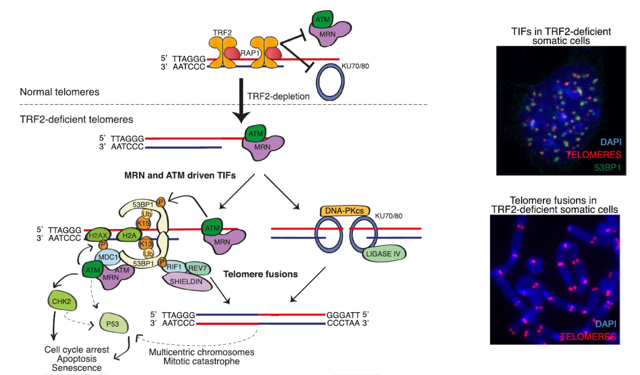
\includegraphics[width=0.5\textwidth]{../_resources/Screen_Shot_2022-12-15_at_17-49-51.png}
\caption{Screen Shot 2022-12-15 at 17-49-51.png}
\end{figure}

The shelterin proteins inhibit DNA damage response and DNA repair
mechanisms at chromosome ends. A key function of telomeres is to inhibit
DDR and DNA repair pathways at chromosome ends. By blocking shelterin
proteins, we reach \emph{senescence} (does not allow cell division,
incompatible with survival) or apoptosis, or chromosome fusions.

\begin{figure}
\centering
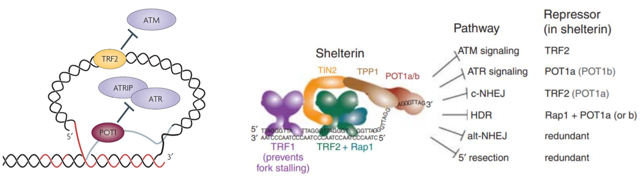
\includegraphics[width=0.5\textwidth]{../_resources/Screen_Shot_2022-12-15_at_17-49-02.png}
\caption{Doksani \& de Lange. \emph{Cold Spring Harbor Press.} 2014
Nature Reviews Cancer, 2008}
\end{figure}

Doksani \& de Lange. \emph{Cold Spring Harbor Press.} 2014 Nature
Reviews Cancer, 2008

A few points to remember:

\begin{enumerate}
\def\labelenumi{\arabic{enumi}.}
\tightlist
\item
  Chromosome ends are capped by structures called telomeres
\item
  Telomeres are nucleoprotein complexes protecting the extremities of
  chromosomes from being recognized as DSBs (\textbf{The end protection
  problem})
\item
  Telomere function depends on the proper telomere structure and
  telomere binding proteins
\item
  Altered telomere structure leads to dysfunctional telomeres which are
  recognized as DSBs and trigger a DDR leading to senescence or
  apoptosis
\item
  If DDR pathway is impaired now genome instability arises
\end{enumerate}

\hypertarget{end-of-replication-problem}{%
\subsection{End of replication
problem}\label{end-of-replication-problem}}

``The end replication problem'' (eukaryotes have linear chromosomes) :
chromosome ends are not fully copied during DNA replication . Also, the
5' end is shorter than the lagging strand (because the template is
short). In addition, in the lagging strand, the RNA primers do not
anneal exactly at the last nucleosome, leading to uncertainty.

\begin{figure}
\centering
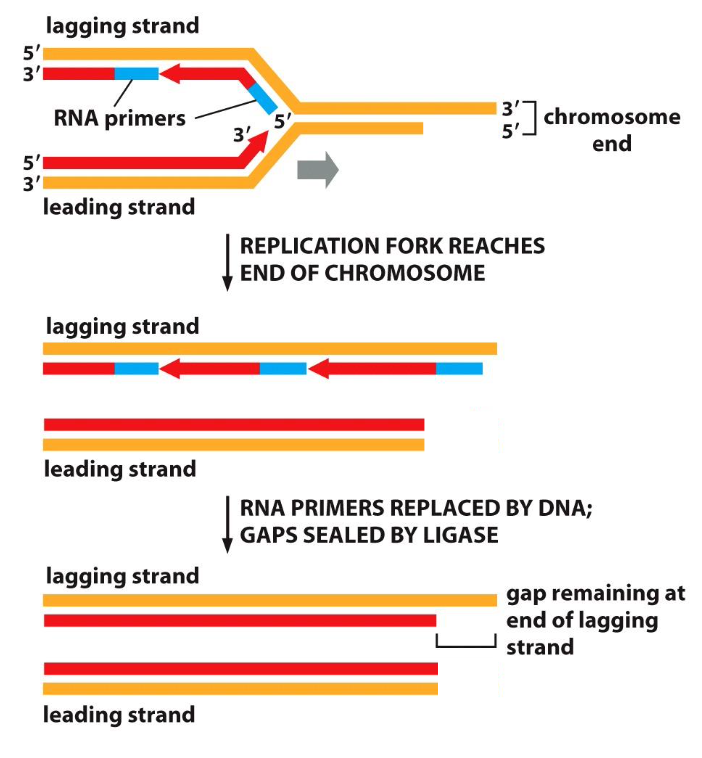
\includegraphics[width=0.5\textwidth]{../_resources/Screen_Shot_2022-12-15_at_18-00-30.png}
\caption{Screen Shot 2022-12-15 at 18-00-30.png}
\end{figure}

Chromosome ends shorten at every cell division: ****the souther it
replicates, the shorter the chromosome end will become, due to an
intrinsic limitation of the DNA replication machinery.

Experimentally, we can check telomere length with:

\begin{itemize}
\tightlist
\item
  \textbf{Southern blot} analyses: genomic DNA is digested with capping
  enzymes, which do not cut inside telomeric repeats → full length
  telomeric sequences. Due to the fact that they are repetitive and
  replication is not complete, the first thing that we can observe is
  that telomere lengths are heterogenous, every telomere has a different
  length (stochastic).
\item
  \textbf{DNA-FISH}: usage of fluorescent probes binding is a sequence
  specific manner, the intensity of the signal is proportional on the
  quantity. The technique is usually applied during metaphase. If we
  were to do this on a population of fibroblasts, we could appreciate
  also the fact that different cells have different telomeres lengths.
\end{itemize}

\textbf{Telomere repeats are lost with age in human leukocytes}: we are
born with a pool of telomeres of a specific size, which will shorten
over time. But the shortening is not linear: 0-1 shortening of 400-500
hundred of bases per year and slows down. The shortening rates are not
even the same for every cells! There's also a sex bias: females have on
average longer telomeres both at birth and throughout life.

Telomeres shorten at each replication cycle up until a threshold, when
DNA breaks are introduced. In human stem cells, this results in a low
self-renewal capacity.

\hypertarget{hayflick-limit}{%
\subsubsection{Hayflick limit}\label{hayflick-limit}}

Discovery by Hayflick in 1961 (Hayflick limit): after a logarithmic
growth, cells reach a plateau. There exists a limited population number
that human cells can go through. The experiment involved fetal stem
cells, with lung cells being the best ones at diving. Inverse
correlation of age of the donor with max population doubling was
observed. \textbf{Telomere shortening associates with decreased
proliferative capacity of cells.}

\begin{itemize}
\tightlist
\item
  Telomere length correlates with the proliferative capacity of cells =
  our biological clock.
\item
  Cells with short telomeres enter senescence earlier than cells with
  longer telomeres.
\end{itemize}

Subsequent ChIP-on-chip experiments confirmed the presence of DNA damage
at the ends of chromosomes in senescent cells. Also, by removing
repairing pathways, it was found that cell cycle arrest in senescent
cells depends on DNA damage response pathways.

\hypertarget{triggering-senescence}{%
\subsubsection{Triggering senescence}\label{triggering-senescence}}

It's not actually the length of the telomeres that induces
\emph{senescence}, but their \emph{structure}. If we find a way to
promote t-loop formation, we can postpone senescence.

Study: TRF2 increased expression on telomeres promotes telomeres
shortening with a higher shortening rate - probably because of a more
stable t-loop, which impairs replication. Since telomeres are shorter,
we expect that they enter early senescence, but this is not observed →
senescence entrance does not depend on telomere length. It is the
altered structure triggering the activation.

Somatic cells will normally grow and reach the Hayflick limit,
triggering senescence. However, if we remove p53/Rb, we reach a M2
crisis, with increased genetic instability. The cells cannot sustain so
much genome instability, so they die because of the crisis. Replicative
senescence and crisis are two proliferative barriers controlled by
telomere deprotection.

It is thought that there are intermediate states of telomere length,
long enough to activate DNA damage response (sensed by cells) but not to
fusion (not short enough to cause disruptive events, uncapped).
Intermediate states are still kind of able to recruit the sheltering
complex.

\begin{figure}
\centering
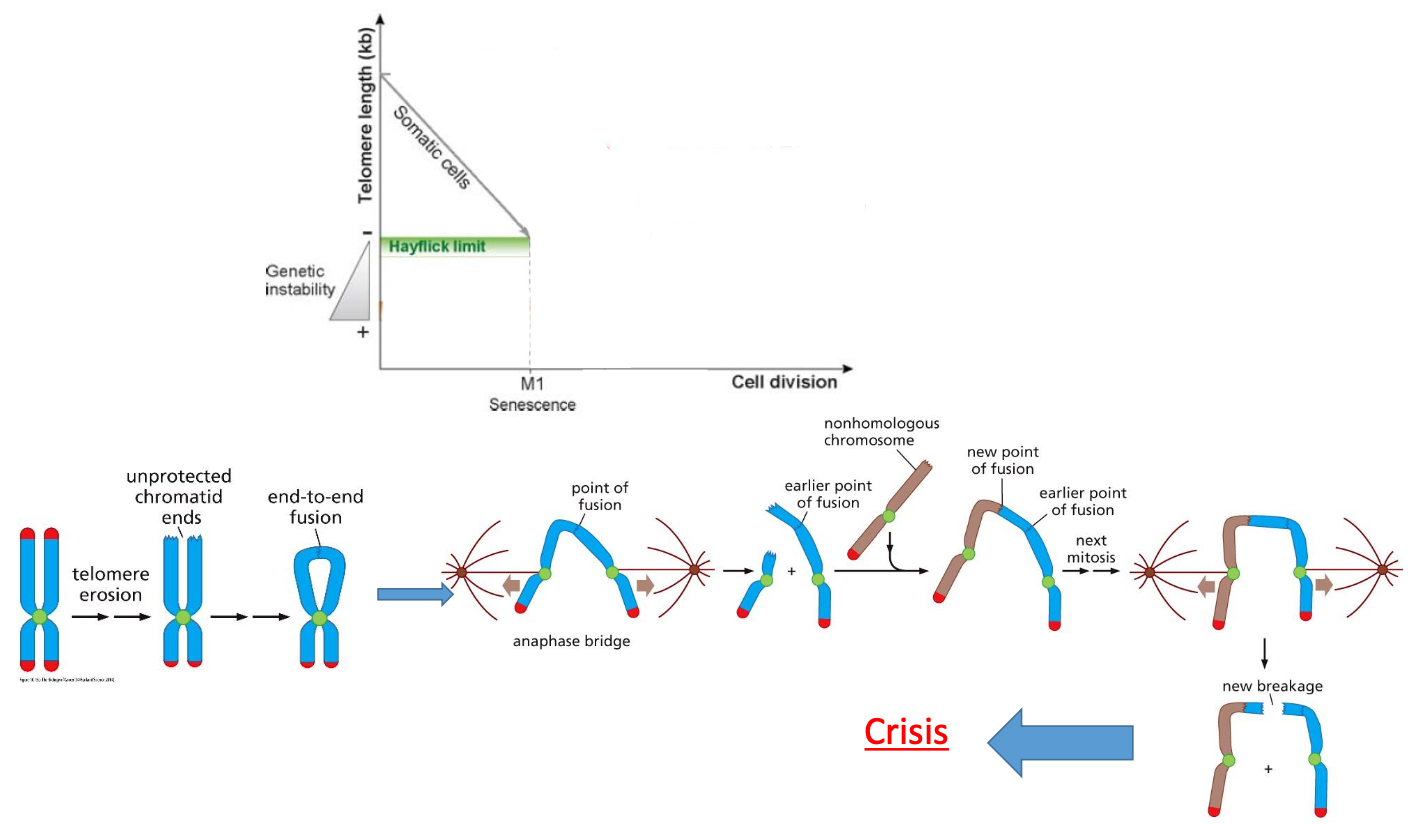
\includegraphics[width=0.5\textwidth]{../_resources/Screen_Shot_2022-12-15_at_22-39-00.png}
\caption{Stewart \& Weinberg. Ann Rev Cell Dev Biol, 2006}
\end{figure}

Stewart \& Weinberg. Ann Rev Cell Dev Biol, 2006

Replicative senescence and crisis are independent cellular programs
induced by distinct telomere states and associated with distinct
biological outcomes.

\hypertarget{cell-crisis}{%
\subsection{Cell crisis}\label{cell-crisis}}

It is not yet clear how a cell crisis occurs (no p53 dependent death).
When cells approach crisis, by bypassing senescence, the time of mitosis
is extremely elongated: \emph{mitotic arrest} (from 30mins to hours).

During the \textbf{mitotic arrest,} we are at the spindle assembly
checkpoint, chromosomes are not properly attached by the two opposite
spindles. Due to the genomic instability provoked by short telomeres,
mitotic arrest amplifies telomeric deprotection, fostering the crisis.

The way cells die is only now being discovered: during the prolonged
mitotic arrest exposed DNA activates DNA sensing mechanisms, triggering
a particular kind of \textbf{autophagic cell death}. Telomeric DNA
damage generates cytosolic DNA species with a fragile nuclear envelopes
that undergo spontaneous disruption. The cytosolic chromatin fragments
activate the cGAS-STING pathway and engage the autophagy machinery,
which is an integral component of the tumor suppressive crisis
mechanism.

\hypertarget{telomerase-enzyme}{%
\subsection{Telomerase enzyme}\label{telomerase-enzyme}}

Stem cells need to undergo hundreds of cell divisions without stressing
out. How can they do it?

In 1995, Greider and Blackburn managed to identify a specific telomere
terminal transferase activity in Teatrahymena (thermophile). In
thermophiles, there are a lot of very little chromosomes, with many
telomeres. When they incubated oligonucleotides with the sequence of the
telomeres, they observed elongated. An enzyme goes and duplicates it
also adding six more nucleotides. This could not be done with a regular
RNA polymerase, there is no template: the enzyme is perceiving and
elongating the sequence.

They found out that there exists an enzyme which also provides for the
template.

\begin{figure}
\centering
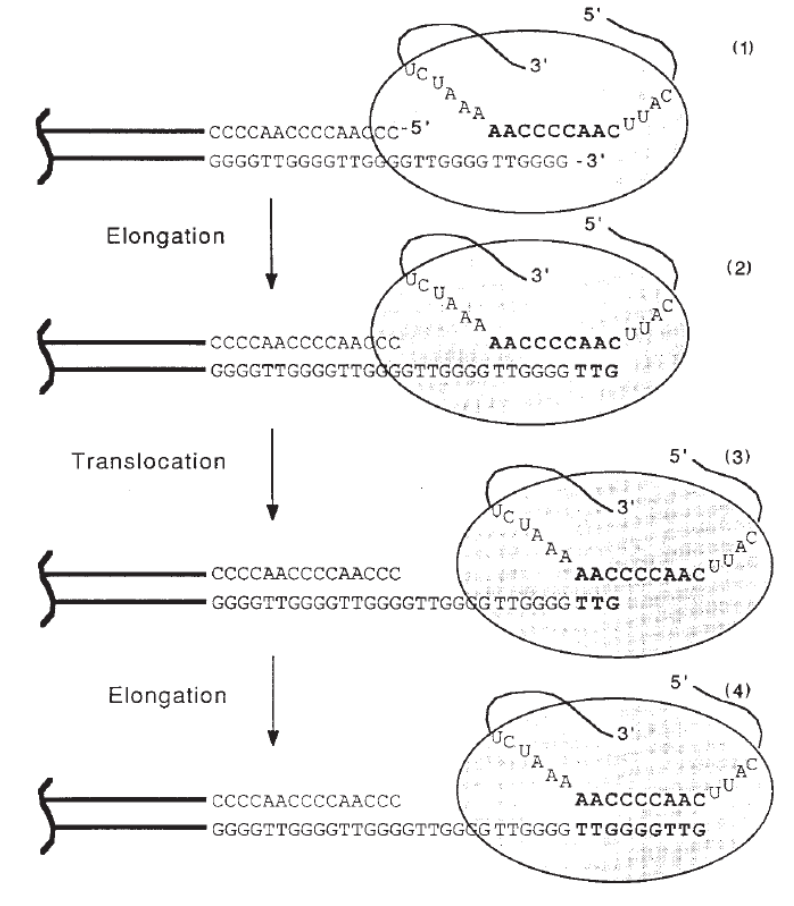
\includegraphics[width=0.5\textwidth]{../_resources/Screen_Shot_2022-12-15_at_22-58-03.png}
\caption{Screen Shot 2022-12-15 at 22-58-03.png}
\end{figure}

In addition to the shelterin complex, also telomerase enzyme is
recruited on telomeric DNA. The telomerase RNA (TR) acts as a scaffold
module for telomerase assembly. The template is 11 bases long. The RNA
feature the presence of H-box domain, aiding in the recruitment of
TCAB1.

\begin{figure}
\centering
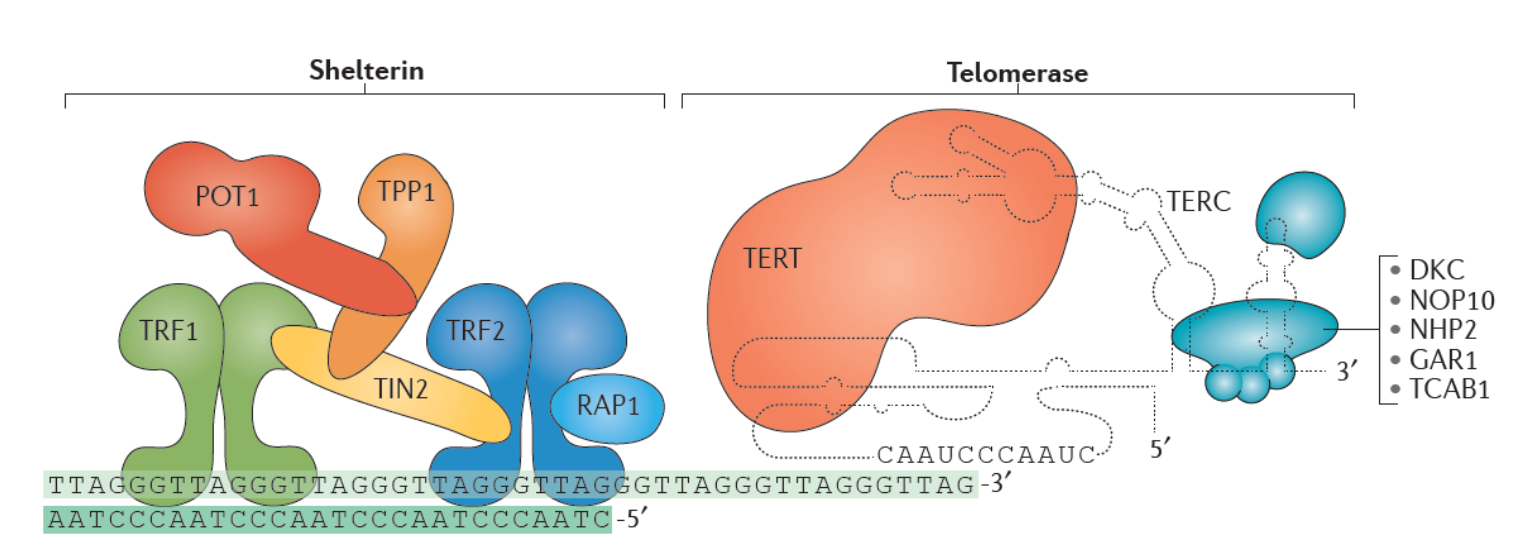
\includegraphics[width=0.5\textwidth]{../_resources/Screen_Shot_2022-12-15_at_22-58-28.png}
\caption{Screen Shot 2022-12-15 at 22-58-28.png}
\end{figure}


Just after birth, telomerase activity drops. Some telomerase activity
can only be found in germ cell production (testicles). Telomerase
elongates telomeres in a stepwise manner, processive enzyme. Once it is
recruited, it is able to add 6-mers (not only 6 nts).

We also need to generate the second strand of telomeric DNA, since the
sheltering complex is recruited on dbDNA. Almost all eukaryotes use
telomerase to elongate telomeres.

\hypertarget{usage-of-telomerase}{%
\subsubsection{Usage of telomerase}\label{usage-of-telomerase}}

``Creation of human tumor cells with defined genetic elements'':
overexpressed hTERT to make up for telomere shortening, immortalization
(inhibition of p53 and Rb).

Mutations in TERT promoter represent the most frequent noncoding
mutations in cancer.

A DNA double strand break (DSB) generates new chromosome ends
structurally similar to a telomere.
